\documentclass[12pt,letterpaper]{article}
\usepackage{natbib}

%Packages
\usepackage{pdflscape}
\usepackage{fixltx2e}
\usepackage{textcomp}
\usepackage{fullpage}
\usepackage{float}
\usepackage{latexsym}
\usepackage{url}
\usepackage{epsfig}
\usepackage{graphicx}
\usepackage{amssymb}
\usepackage{amsmath}
\usepackage{mathtools}
\usepackage{bm}
\usepackage{array}
\usepackage[version=3]{mhchem}
\usepackage{ifthen}
\usepackage{caption}
\usepackage{hyperref}
\usepackage{amsthm}
\usepackage{amstext}
\usepackage{enumerate}
\usepackage[osf]{mathpazo}
\usepackage{dcolumn}
\usepackage{lineno}
\usepackage{dcolumn}
\newcolumntype{d}[1]{D{.}{.}{#1}}

\pagenumbering{arabic}


%Pagination style and stuff
\linespread{2}
\raggedright
\setlength{\parindent}{0.5in}
\setcounter{secnumdepth}{0} 
\renewcommand{\section}[1]{%
\bigskip
\begin{center}
\begin{Large}
\normalfont\scshape #1
\medskip
\end{Large}
\end{center}}
\renewcommand{\subsection}[1]{%
\bigskip
\begin{center}
\begin{large}
\normalfont\itshape #1
\end{large}
\end{center}}
\renewcommand{\subsubsection}[1]{%
\vspace{2ex}
\noindent
\textit{#1.}---}
\renewcommand{\tableofcontents}{}
%\bibpunct{(}{)}{;}{a}{}{,}

%---------------------------------------------
%
%       START
%
%---------------------------------------------

\begin{document}

% To be submitted to MEE as a Mini-review (http://www.methodsinecologyandevolution.org/view/0/authorGuidelines.html)

%Running head
\begin{flushright}
Version dated: \today
\end{flushright}
\bigskip
\noindent RH: Avoiding redundant tree rearrangements

\bigskip
\medskip
\begin{center}

\noindent{\Large \bf A simple rule for avoiding redundant topologies during tree rearrangement procedures} 
\bigskip

\noindent {\normalsize \sc Thomas Guillerme$^1$$^*$, and Martin D. Brazeau$^1$}\\ %TG: Author order can be swapped of course! There's only a finite combination of 2 elements anyway!
\noindent {\small \it 
$^1$Imperial College London, Silwood Park Campus, Department of Life Sciences, Buckhurst Road, Ascot SL5 7PY, United Kingdom.\\}
\end{center}
\medskip
\noindent{*\bf Corresponding author.} \textit{t.guillerme@imperial.ac.uk}\\  %TG: Same as above
\medskip
Word count: @@@
\vspace{1in}

%Line numbering
\modulolinenumbers[1]
\linenumbers

%---------------------------------------------
%
%       ABSTRACT
%
%---------------------------------------------

\newpage
% \begin{abstract}
\section{Abstract}
\begin{enumerate}
    \item Tree rearrangement methods are central to evolutionary biology, whether used during or after phylogenetic inference. They are well described in the literature both in terms of algorithm descriptions and caveats studies. However, following these instructions generates redundant rearrangements. %Point 1: set the context and purpose for the work;
    \item In this review, we propose an approach that allows to perform the most used tree rearrangement methods (SPR/TBR) without obtaining redundant trees.%Point 2: indicate the approach and methods used;
    \item Although this method is probably already implemented in phylogenetic software, this is the first paper to propose a simple and easily implementable solution that could be used by software engineers in the future. %Point 4: identify the conclusions, the wider implications and the relevance to management or policy. 
\end{enumerate}
% \end{abstract}

\noindent (Keywords: Subtree Pruning and Regrafting, Tree Bisection and Reconnection, Heuristic search algorithm, tree topology)\\

\vspace{1.5in}

\newpage 

%---------------------------------------------
%
%       INTRODUCTION
%
%---------------------------------------------
\section{Introduction}

% Tree rearrangement is paramount
Phylogenetic tree inference methods are confronted with the combinatoric problem of unmanageable large numbers of tree solutions arising from increasing numbers of terminals \citep{Felsenstein:1978vh}.
To address this problem, heuristic solutions involving tree rearrangements allows exploration of restricted parts of the ``tree space'' close to target solutions.
This greatly accelerates phylogenetic analysis by ignoring topologies that are unlikely to be optimal.
In addition to their use in phylogenetic tree search process itself, tree rearrangement strategies are employed in some post-search tasks such as tree comparisons \citep[e.g.][]{allen2001subtree,kuhner2015treComparison}, node support estimation \citep[e.g.][]{goloboff2014bias} or methods for detecting horizontal genes transfer \citep[e.g.][]{mcfadden1995something,bordewich2005computational}.

Recently, \citet{goloboff2014bias} examined biases in tree searches arising from heuristic methods, noting in particular how these biases can influence support statistics including bootstrap values and posterior probabilities arising from Bayesian inference.
They note that the biases are amplified if tree rearrangement %TG: I've standardised "branch-reinserting" to "tree rearrangement" for consistency
procedures do not take care to avoid redundant rearrangements. %TG: I've standardised "swaps" to "rearrangement" for consistency
Additionally, because tree rearrangement strategies are at the base of any phylogenetic studies, their speed and efficiency are of critical importance.
Considerable time should be saved by not visiting topologies that have already been analysed.
Although tree rearrangement strategies have been well studied in the literature, the question of how redundant rearrangements are avoided may not be immediately obvious from the explanations given in most texts \citep{swofford2003phylogeny,felsenstein2004inferring,wiley2011phylogenetics}.
In fact, the explanations given for tree rearrangement algorithms (reviewed below) given in most popular texts and reviews will almost certainly result in redundant topologies within even the same round of branch reinserting.

How then are redundant rearrangements avoided?
In this review, we provide more intuitive explanations of the subtree pruning and regrafting (SPR) and tree-bisection and reconnection (TBR) rearrangement strategies that result only in unique tree topologies within a single round.
These explanations account for the order in which branches are broken as well as the pattern in which subtrees are reconnected to the target subtree.
We do not claim credit for these methods; they, or something equivalent to them must already be implemented in existing phylogenetic software.
Furthermore, they are implicit in some mathematical accounts of tree rearrangement processes in which the number of unique 1-move rearrangements are counted \citep{allen2001subtree}.
However, we provide an explicit, verbose account that would be useful in assisting any investigators who need to program such routines for the first time. 
We acknowledge that few may need to do this, however we follow \citet{goloboff1993character} in that knowledge of underlying routines helps to foster refinements and improvements of existing strategies that have a large user base.
%TG: not sure about the "few needs to know" part. It's kind of auto-diminishing the impact of the paper. We should proprably go with something more grandios!


% %MB I'm really not sure this section is needed, but I'll leave it for now. It might be possible to fit it in.
% %MB For now, it's mainly a digression from the main point: only unique 1-move rearrangements from a starting tree. TG: I've move that where it could fit.

\section{SPR and TBR described in literature}
The tree inference literature contains thorough and precise descriptions of both the SPR and TBR algorithms \citep[e.g.][]{allen2001subtree,felsenstein2004inferring} and their caveats \citep[i.e speed and reliability - e.g.][]{morrison2007increasing,lakner2008efficiency,goloboff2014bias}.
%TG: possible disgression:
% Two main points need to be considered for the reliability of tree arrangement algorithms:
% \begin{enumerate}
%     \item First, when the tree search only visits some possible solutions this can create problems by having a higher probability of visiting a specific tree topology island since the probability of obtaining any topology by tree rearrangement will not be equal (some topologies might be more visited by chance).
%     More concretely, for a tree with $n$ taxa, tree rearrangement algorithms can produce $M$ topologies including $m$ similar ones.
%     If the tree search algorithm is set to subsample $m$ topologies only, it can possibly only subsample the $m$ similar topologies thus being ineffective at exploring tree space \citep{allen2001subtree}.
%     \item Second, the order in which the possible tree rearrangement topologies are visited is also paramount.
%     In fact, to avoid any statistical bias, the visiting order should be strictly random \citep{goloboff2014bias} although, in practice, and for algorithm speed reasons, this is rarely the case (e.g. using post/pre-order traversals [CITE]).
%     This as been shown to introduce several biases in theoretical examples \citep{goloboff2014bias} although, to our knowledge, has not been demonstrated empirically.
% \end{enumerate}
However, the description of the \textit{implementation} of the algorithms is often overlooked.
% Here, we will review these two tree rearrangement strategies and propose a more practical and intuitive definition of the algorithms that we believe can help their implementation.
% It is important to note that the algorithms described here are mathematically equivalent to the ones described in \cite{allen2001subtree} and \cite{felsenstein2004inferring} and we thus do not claim priority or originality on this method that as certainly already be implemented in many softwares and was ``discovered'' empirically by many coders.
% TG: is that bit not repeated in the paragraph above?
The SPR method is commonly described as breaking a tree into to two subtrees and reinserting one of these subtrees -- the source subtree see \hyperref[Glossary]{Glossary}%TG: I've standardised "tree" to "subtree" in the context of source/target subtrees.
-- into all non-redundant positions on the other subtree -- the target subtree (see \hyperref[Glossary]{Glossary}).
In some explanations the target subtree is then reinserted into all available positions on the source subtree \citep[e.g.][Fig. 8.5]{swofford2003phylogeny}.
However, if all possible subtrees are broken and reinserted (see \hyperref[Glossary]{Glossary}) %TG: standardised "breaking" to "breaking" and "reinserting" to "reinserting"
 exactly according to the rules described, then they will always generate redundant trees (Fig. \ref{Figure_redundant}). 
In many cases, branch breaking and reinsertion would continue, long after the number of non-redundant topologies has been exhausted, wasting valuable computational time and biasing the tree search \citep{goloboff2014bias}.

TBR differs from SPR in that the source subtree is rerooted before reconnection to the target subtree.
Thus TBR can be seen as a generalisation of SPR where, in the latter, the source subtree is left rooted on the breaking point.
All possible rerooting of the source subtree are attempted before the next breaking is made.
Because the SPR is a strict subset of TBR moves on any given bifurcating tree, then the problem described here holds as well for TBR.
In either case, it is clear that not all possible branch breaking and reinsertions need to be attempted.

% \section{The Target and source subtree} TG: I've moved that in the glossary

\section{Patterns Generating Redundant rearrangements}
The most obvious case in which a breaking and reconnection procedure results in a redundant topology is the case of reinserting the source subtree to its original position on the target subtree.
If avoiding this operation is trivial, figure \ref{Figure_redundant} shows three different breaking and reconnection operations that avoid the original reinsertion point but still result in the same topology. 
From the figure, one can notice that one of their commonality is that all these reinsertions are done on the branch neighbouring the original position (see \hyperref[Glossary]{Glossary}).
%This clips the tree at the smallest subtree that includes both clades. %MB: This is possibly coincidental, but possibly also work thinking about. TG: not sure I get you here?
Rerooting any of these source subtrees on the branch subtending terminal ``C'' and reinserting it to the original breaking branch will also generate the same topology.
Conversely, this can be seen as breaking the clade consisting of terminals ``A'' and ``B'' and reinserting that clade on its neighboring branch (the one subtending ``C'').
%TG: not sure also what you meant in this part? Is this for illustrating another example (the same source trees rerooted on the branch to C?) or did you mean that it does the same on other neighbouring positions?
All of these redundant rearrangements arose from the breaking and moving of the source subtree to a neighbouring branch of the breaking point on the target tree.
In the next section we show how to employ the order of breaking so that only one of these rearrangements is made even when the same breaking event occurs.

\begin{figure}[!htbp]
\centering
   \includegraphics[width=0.9\textwidth]{Figure/Figure_Redundantswaps.pdf}
\caption{Example of redundant rearrangements. Three independent breaks (clades ``(A,B)'', ``(G,F)'' and ``(E,D)'') and reconnection (orange doted line) leading to the same topology. The big orange dots represents the clade's original position.}
\label{Figure_redundant}
\end{figure}

\section{Avoiding Redundant rearrangements}
As described above and illustrated in figure \ref{Figure_redundant}, some breaking and reconnection can result in the same tree topology if the reconnection is done in the neighbouring branches of the insertion point.
To avoid these redundant rearrangements, we thus only need to commit one of these moves once.

In SPR moves, when a branch is broken, the source subtree is reinserted everywhere except on the original breaking branch \textit{and} any branches immediately adjacent to the original site. 
In turn then, the target subtree (containing the traversal starting point) is reconnected to the source subtree at all possible points \textit{including} branches neighbouring the original breaking branch.
This rule can be also applied to the TBR algorithm, however, when the source subtree is rerooted, it must be reinserted to the original breaking point on the target subtree \textit{and} the branches adjacent to it (see Fig.\ref{Figure_Neighbor}).

\begin{figure}[!htbp]
\centering
   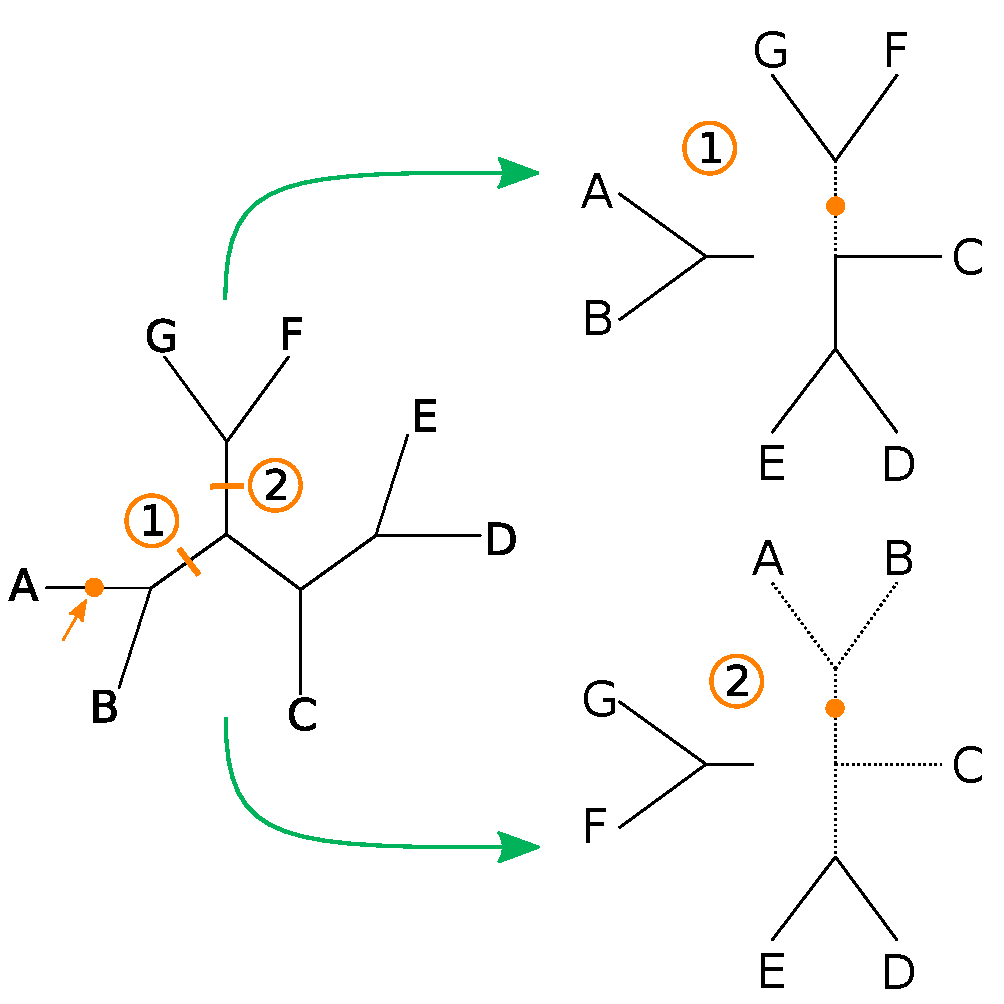
\includegraphics[width=0.7\textwidth]{Figure/Figure_Neighbour.pdf}
\caption{Algorithm illustrating how to avoid redundant rearrangements. If the starting point in the traversal is on the tip ``A'' (denoted by the orange arrow), the clade containing the entry point (e.g. ``(A,B)'') can be rebranched everywhere on the target subtree (the black solid edges) apart from it's previous position (the orange doted line). Any other clades not containing the entry point (e.g. ``(F,G)'') can only be rebranched on edges not adjacent to the original position.}
\label{Figure_Neighbor}
\end{figure}

Using this simple rule during any tree rearrangement algorithm using the SPR or/and TBR routines allow to properly explore the tree space \citep[i.e. the correct number of topologies are visited, following][]{allen2001subtree} without any redundant tree rearrangement.

% TG: actually need to check that.
% number of splits = 2n-3
% number of reinsertions = 2n−4

% number of reinsertions = 2n-4-5 (5 is )

% operation 3 = 4(n−3)(n−4)
% (4n-12)*(4n-16)

% 4n^2-64n-48n-192
% 4n^2-16n-192


% NNI rearrangements: 2(n-3)

% 2(n-3) + 4(n−3)(n−4)

% Result = 2(n−3)(2n−7)
% (2n-6)*(4n-14)


% One major concern in phylogenetic inference, during the tree search phase is to evenly (or at worst, randomly) sample the tree space but without spending to much time sampling all possible topologies.
% This allows to identify the different topology islands where the tree search must be focused in order to find the optimal topology.
% One solution to achieve this it to shift between tree rearrangement algorithms during the tree search: first, using an algorithm allowing bold tree rearrangements to explore the overall tree space and then a more conservative one to do a ``fine grain'' search in local optima \citep{lakner2008efficiency}.
% This joint SPR-TBR implementation could easily allow such tree rearrangement shifts by switching between the different restriction rules without implementing different algorithms.
% For example, one could first allow the algorithm to reroot the bissected tree randomly on each of it's edges, creating bolder rearrangements (i.e. exploring the overall tree space) and the constrict the algorithm to only reroot the tree on the edge closest to the bisection edge, creating ``finer grain'' search (i.e. exploring only the SPR island).


% % Dunno if we'll keep the stuff below ##################
% % ######################################################
% \section{Implementation spin}
% These two algorithms can be seen as technically different since they will produce different tree islands, for example, the SPR will, in theory explore fewer topologies than the TBR \citep[see above and][]{morrison2007increasing,lakner2008efficiency}.
% However, once one excludes the visiting of redundant topologies in both algorithms, they can be seen as a generalised way to explore effectively all possible tree topologies.
% First, as described in \cite{allen2001subtree} (but not in \citealt{felsenstein2004inferring}), a simple rule can be applied to avoid redundant topologies in both SPR and TBR algorithm: in both cases the rebranching/reconnection should never occur on the edge of origin (the red arrow in Figs %\ref{Figure_SPR}, \ref{Figure_TBR} and \ref{Figure_TBR_modif}
% ) but neither on the neighbouring ones \citep{allen2001subtree}.
% Second and foremost, an SPR algorithm can be implemented as a TBR one where the rerooting is only done on the edge the closest to the bisection point.% (see Fig \ref{Figure_TBR_modif}).

% % \begin{figure}[!htbp]
% % \centering
% %    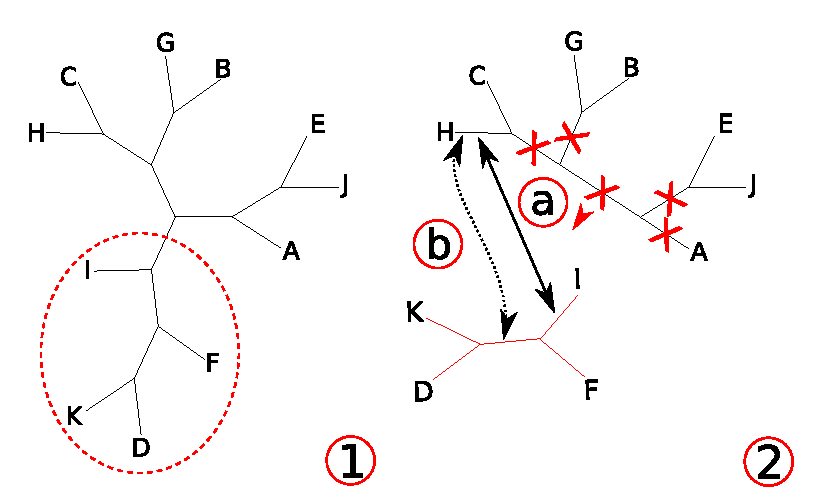
\includegraphics[width=0.9\textwidth]{Figure/TBR_modif.pdf}
% % \caption{Generalised TBR. \textbf{1}: the trees are split at a random edge and both subtrees are unrooted; \textbf{2a}: the red tree is then rooted on the edge closest to the bisection edge and reconnected to an edge on the black tree (i.e. a SPR move); \textbf{2b}: the red tree is rooted on any of its edges and reconnected to an edge on the black tree (i.e. a TBR move). Note that in both cases, the red tree can not be reconnected on the edge of origin (indicated by the red arrow) nor on any of the adjacent edges (marked with a red cross) to avoid any redundant tree rearrangements.}
% % \label{Figure_TBR_modif}
% % \end{figure}



% We believe that such consideration of the SPR algorithm as a constrained TBR highly facilitates both algorithm's implementation.
% In fact, in this case only one algorithm needs to be implemented with one mandatory restricting rules (no reconnection on the bisection edge and it's neighbours) and an optional restriction that can be activate or not to create either TBR or SPR (respectively rerooting on any edge or only on the bisection one).
% This approach is not different than the classic SPR and TBR algorithms described in the literature \citep{allen2001subtree,felsenstein2004inferring} but proposes an easier implementation.

% One of the major concern in phylogenetic inference, during the tree search phase is to evenly (or at worst, randomly) sample the tree space but without spending to much time sampling all possible topologies.
% This allows to identify the different topology islands where the tree search must be focused in order to find the optimal topology.
% One solution to achieve this it to shift between tree rearrangement algorithms during the tree search: first, using an algorithm allowing bold tree rearrangements to explore the overall tree space and then a more conservative one to do a ``fine grain'' search in local optima \citep{lakner2008efficiency}.
% This joint SPR-TBR implementation could easily allow such tree rearrangement shifts by switching between the different restriction rules without implementing different algorithms.
% For example, one could first allow the algorithm to reroot the bissected tree randomly on each of it's edges, creating bolder rearrangements (i.e. exploring the overall tree space) and the constrict the algorithm to only reroot the tree on the edge closest to the bisection edge, creating ``finer grain'' search (i.e. exploring only the SPR island).


\section{Glossary}
\label{Glossary}
% Standardisation: site becomes branch in the context of neighboring or breaking sites/branches.
% Rearangements/Swap to be standardised?

\begin{itemize}
    \item{\textbf{breaking branch}: branch where the \textbf{Parent tree} is divided into the \textbf{target subtree} and the \textbf{source subtree}.}
    \item{\textbf{Neighboring branches}: all branches that are connected by one node to the \textbf{breaking branch} (i.e. the branches directly adjacent to it).}
    \item{\textbf{Parent tree}: the complete tree that undergoes branch rearrangement (i.e. the input tree).}
    \item{\textbf{Reinsertion}: the branch where the \textbf{target subtree} is reinserted on the \textbf{source subtree}.}
    \item{\textbf{source subtree}: the subtree issue from the \textbf{breaking} that does \textit{not} contains the \textbf{starting point}.}
    \item{\textbf{Starting point}: the branch leading to the terminal where the post/pre-order traversal algorithm is initiated.}
    \item{\textbf{target subtree}: the subtree issue from the \textbf{breaking} that \textit{does} contains the \textbf{starting point}.}
    \item{\textbf{post/pre order traversal}: }
\end{itemize}

\subsection{The source and target subtrees}
% MDB: At this point, it comes clear to me that a glossary or box text might be a useful supplement to define some terms. Secondly, it will be good for us to settle on a few terms and standardise them across the MS.
Although not all breaking and reinsertion points need to be attempted during a branch rearrangement, all possible non-unique moves do need to be tried to make the search properly heuristic. 
The required breakings (or the enumeration of the possible breaking points) can be made bu completing a tree traversal over the initial parent tree (see \hyperref[Glossary]{Glossary}).
In practice, because the parent trees are usually unrooted during the heuristic search, an arbitrary starting points needs to be selected.
For the purpose of this paper, we elect the node immediately adjacent to the first enumerated tip (usually tip ``A'' or ``1'') thus making the trees implicitly rooted by the traversal procedure.
Breaking may then proceed either in postorder or preorder %TG: do these needs to be explained?
, but in either case, the recursive traversal concludes at the node in which the traversal was initiated.

Because the tree is now implicitly rooted, we can properly define the target and source subtrees for SPR and TBR with respect to this pattern.
For the purposes of this paper, the target subtree is the subtree that contains the starting point of the tree-breaking traversal.
By extension, therefore, the source subtree is the broken subtree that does not contain the starting point.

%TG: Fair enough for the Glossary. Although if we decide to go for it properly, this section should be removed. It'll also make the reading flow much nicer: 1 - SPR TBR in litterature; 2 - what creates redundant swaps; 3 - our implementation to avoid it.





\section{Acknowledgments}
European Research Council under the European Union’s Seventh Framework Programme (FP/2007–2013)/ERC Grant Agreement number 311092.



\bibliographystyle{sysbio}
\bibliography{References}

% Original tree: the tree considered for branch reinserting operation
% broken tree: the sub-tree containing one to n-2 taxa removed from the original tree
% target subtree: the tree that underwent a breaking operation and has now n-1 to n-(n-2) taxa. %TG: we could change that to a more obvious term
% breaking (to replace: prunning or bissection): removing a sub-tree containing one to n-2 taxa from a tree. The breaking results in obtaining two trees: the broken tree and the target subtree.
% Regrafting/reconnecting: %TG: we should change that to a unique term (same way as breaking, I like reconnecting).
% Swap: one breaking regrafting operation
% Neighbour edge: the edge adjacent to a selcted edge



\end{document}

